\documentclass {amsart}

\usepackage{graphicx}
\usepackage{listings}
\usepackage{color}
\usepackage{verbatim}
\usepackage{hyperref}


\definecolor{lightgray}{rgb}{.9,.9,.9}
\definecolor{darkgray}{rgb}{.4,.4,.4}
\definecolor{purple}{rgb}{0.65, 0.12, 0.82}

\lstdefinelanguage{JavaScript}{
  keywords={typeof, new, true, false, catch, function, return, null, catch, switch, var, if, in, while, do, else, case, break, try},
  keywordstyle=\color{blue}\bfseries,
  ndkeywords={class, export, boolean, throw, implements, import, this},
  ndkeywordstyle=\color{darkgray}\bfseries,
  identifierstyle=\color{black},
  sensitive=false,
  comment=[l]{//},
  morecomment=[s]{/*}{*/},
  commentstyle=\color{purple}\ttfamily,
  stringstyle=\color{red}\ttfamily,
  morestring=[b]',
  morestring=[b]"
}

\lstset{
   language=JavaScript,
   %backgroundcolor=\color{lightgray},
   extendedchars=true,
   basicstyle=\footnotesize\ttfamily,
   showstringspaces=false,
   showspaces=false,
  % numbers=left,
   numberstyle=\footnotesize,
   numbersep=9pt,
   tabsize=2,
   breaklines=true,
   showtabs=false,
   captionpos=b
}



\title {Introduction to JavaScript}


\begin{document}

\maketitle

\section {History}

\begin{itemize}
	\item Created at Netscape
	\item Originally written in 1995 by Brandon Eich
	\item Called JavaScript to entice Java developers to try it.  (It's more like LISP than C.  Don't be fooled.);
	\item Microsoft reverse engineered the language for integration into Internet Explorertext
	\item Become ECMA Script in 1997 and is when Netscape lost control. 
\end{itemize}


\section{Coding Standards}
	\subsection{JsLint}
		Before programming download and install JSLint.  There is an addon to Visual Studio under: Tools - Extensions and Updates
		\\
		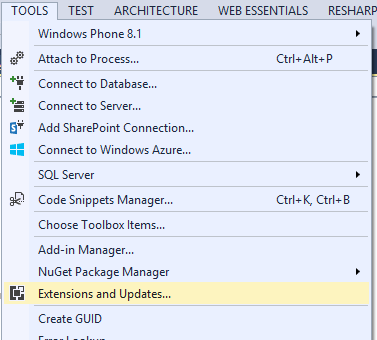
\includegraphics[scale=.75]{ToolsExtensionsAndAddons.png}
		\\
		\\
		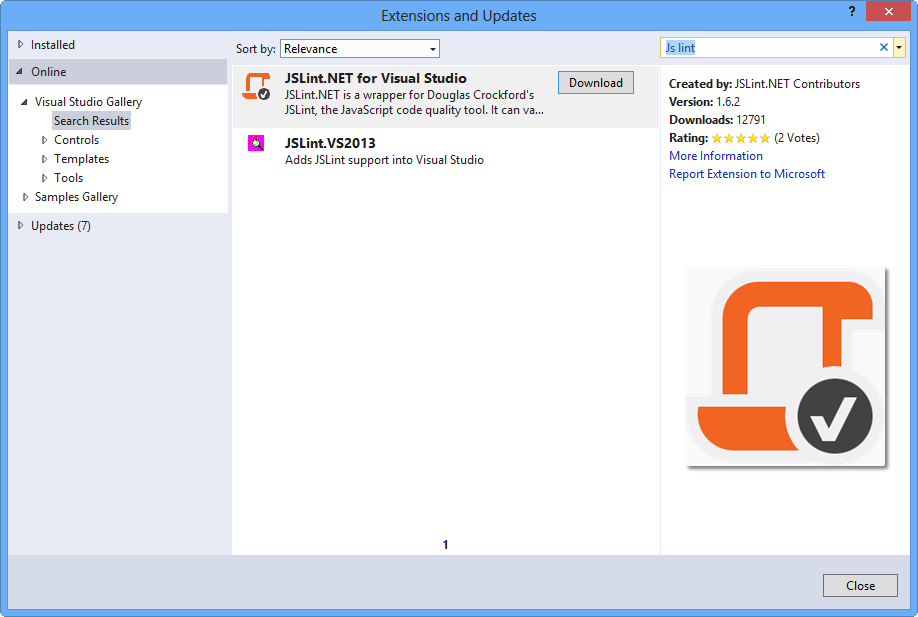
\includegraphics[scale=.45]{JsLintAddOn.png}
	\subsection {Brackets}

		Always put brackets on the same line as the conditional or the return statement.

		\begin{lstlisting}
			function myFunction () {
				//your code here;

				return {};
			}
		\end{lstlisting}	

		JavaScript sees a carriage return as a statement ending.

\section {Functions}
	There are two ways of creating a function:

	\begin{lstlisting}
		function myName (){
			//your code here
		}
	\end{lstlisting}

	and 

	\begin{lstlisting}
		var myName = function (){
			//your code here
		}
	\end{lstlisting}

	They both create usable functions, but the first has interpreter validation points built in.  With the second example, JavaScript code cannot call a function assigned to a variable until the variable has been instantiated and assigned the function.  
It must precede any code calling it.  In the first approach, it can exist anywhere in the program.  JavaScript will parse all programs and load the functions into memory before running code.  

	\subsection{Functions First Class Objects}  Functions are objects.  This means that you can return them from functions, and pass them into other functions as arguments.

		
\includegraphics{FunctionAsArgumentsBadTime.jpg}


\section{Statement Endings}
	\subsection{Semicolons}
		This is the optimal way of ending a statement.  Always use this.
	\subsection {Carriage Return}
		A carriage return will end a statement.  This happens by JavaScript inserting a semicolon when it encounters an error.  If this corrects the error, then JavaScript assumes that not having a semicolon was the cause and continues on. 
	\subsubsection {Return Statements With Carriage Returns}
		Since JavaScript will accept a carriage return as a statement ending the two examaples return different results: 
		\begin{lstlisting}
			function foo () {

				return {
					personId:1,
					personName:"Steve"
				};

			}
		\end{lstlisting}
		and
		\begin{lstlisting}
			function foo () {

				return 
				{
					personId:1,
					personName:"Steve"
				};

			}
		\end{lstlisting}
	In JavaScript functions can return undefined so {\bf return;} or {\bf return (carriage return)} is valid, so the second function is legal and returns undefined even though the author intended a new object to be returned instead.

		
\section{Operators}
	\subsection{=== and !==}
		This is the actual comparison operator.  This acts like == in other langauges.
	\subsection{== and !=}
		This does the object on the right hand side of the operator convert to the left.  
		Consider the following: 

		\begin{itemize}
			\item \begin{lstlisting} 
"" == "0" 		//false
				\end{lstlisting} 

			\item \begin{lstlisting} 
0 == '' 		//true
				\end{lstlisting} 

			\item \begin{lstlisting} 
0 == '0' 		//true
				\end{lstlisting} 
		\end{itemize}


		\begin{itemize}
			\item \begin{lstlisting} 
false == 'false' 	//false 
				\end{lstlisting}

			\item \begin{lstlisting} 
false == '0'	 	//true
				\end{lstlisting} 
		\end{itemize}


		\begin{itemize}
			\item \begin{lstlisting} 
false == undefined 	//false
				\end{lstlisting} 

			\item \begin{lstlisting} 
false == null //false
				\end{lstlisting} 

			\item \begin{lstlisting} 
null == undefined //true
				\end{lstlisting} 

			\item \begin{lstlisting} 
' \t \r \n ' == 0 //true
				\end{lstlisting} 

		\end{itemize}

\section{Variables}
	There are two ways of declaring variables in JavaScript 
	/begin{lstlisting}
		var myVariable = "Foo";
	/end{lstlisting}

	and 

	/begin{lstlisting}
		myVariable = "Foo";
	/end{lstlisting}
	\subsection{Hoisting}  Always declare variables at the top of a function.  JavaScripts scope declaration is at the function level and not at the branch level.  JavaScript will automatically move the variable declaration to the top of the function if not placed there. For Example: 
	\begin{lstlisting}
		function () {
			if(true === true){
				var myVariable = "Example";
			}
		}
	\end{lstlisting}

Really becomes: 

	\begin{lstlisting}
		function () {
			var myVariable; 
			if(true === true){
				myVariable = "Example";
			}
		}
	\end{lstlisting}
"myVariable" is now accessible to the entire function.  

\section{Functions}
	There are 3 ways to create a function: 
	\begin{itemize}
		\item function foo () /{/}
		\item var foo = function () /{/}
		\item function () /{/} //anonymous
	\end{itemize}
	\subsection{Variable Length Arguments}  When calling a function, the number of supplied arguments is not enforced.  Missing ones come in as {\bf undefined} and additional ones can be accessed through the {\bf arguments} object. 

	
\includegraphics{MoreArgumentsThanSpecified.jpg}

	\begin{lstlisting}

		function MyShowAllTheArguments (aOne, aTwo, aThree){
			var ii = 0, counter = 0;		
			alert(arguments.length);

			for(ii = 0; ii < arguments.length; ii++){
				counter += arguments[ii];
			}

			alert(counter);
		}

		MyShowAllTheArguments(1,2,3,4,5,6);
		MyShowAllTheArguments(1,2);

	\end{lstlisting}


\section{Primitive Types}
	\subsection{Strings}
			\subsubsection{Escape Characters}

			\begin{center}
			\begin{tabular} {| l |p{5cm}|}
			
				\textbackslash{b} & Backspace \\
				\textbackslash{t} & Tab (horizontal) \\
				\textbackslash{n} & Linefeed (newline) \\
				\textbackslash{v} & Tab (vertical) \\
				\textbackslash{f} & Form feed  \\
				\textbackslash{r} & Carriage return        \\
				\textbackslash{"} & Double quote           \\
				\textbackslash{'} & Single quote           \\
				\textbackslash{}\textbackslash{} & Backslash              \\

			\end{tabular}
			\end{center}
	\subsubsection{Creating an Array}  This is a very fast and convenient way of creating an array.  
		\begin{lstlisting}
			var countries = "U.S.A,Canada,Mexico".split(',');
		\end{lstlisting}
		\begin{itemize}
			\item Less typing.
			\item Less code to screw up.
			\item Easier for other coders to read.
		\end{itemize}
\subsection{Numbers}
	All numbers in JavaScript are 64-bit floating point numbers.  There is no such concept as integer division.  So :  "13 / 3" does not equal 4 but 4.333.... instead.

\subsection {undefined}
	There are three undefined "types" in Javascript 
	\begin{itemize}
		\item Undefined (type)
		\item undefined (value)
		\item undefined (variable)
	\end{itemize}


\subsection {null}


\section{Objects}
	\subsection {Reference Types}
		In JavaScript everything is an object, and all objects are reference types.  There is no pass by value in JavaScript.  
		What this means: 
	
	\subsection{Creating an Object}
		\begin{itemize}
			\item Literal Notation: var o = \{\};
			\item Function: var o = new Object();
		\end{itemize}
		\subsubsection{Constructors} Constuctors are functions with the {\bf new} keyword in front of them.  The {\bf new} operator binds the objesct's prototype to the functions prototype member and bings the object to {\bf this}, instead of binding {\bf this} to the global object.  Common convention is that functions which are to be used as constructors are Pascal Case (First word of each letter is uppercase).  

			\begin{lstlisting}
				function MyNewObject () {
					this.SayHello = function () {
						alert("Hello");
					};
					
					this.PublicProperty = "I am a public property";
				}
			\end{lstlisting}

	\subsection{Arrays}
		\subsubsection {Creating an Array}
			\begin{itemize}
				\item Literal Notation: var arr = [];
				\item Function: var o = new Array();
			\end{itemize}
		Use the literal notation.  There is no benfit to doing {\bf new Array();}.  It just uses extra characters. 
	
	
\section{Script Block}
	In an HTML page each script is a different JavaScript program.  They still share a global namespace {\bf window}, but the failure of one does not affect the other (provided that the second program doesn't rely on parts that weren't executed in the first program due to the failure.)

\begin{lstlisting}
<script>
    my_x = "TEST";

    throw "example";

    function exampleFunction() {
        var myVariable = "";

        alert(myVariable);
    }

    exampleFunction();
</script>
<script>
    alert(my_x);
</script>
\end{lstlisting}
\url{http://jsfiddle.net/X3VdC/1/}

\section{Error Handling}
	\subsection{Try/Catch}   Syntax: 
		\begin{lstlisting}
			try{

			}
			catch(e){
				\\do stuff with e.		
			}
		\end{lstlisting}

\section{JSON : JavaScript Object Notation}

	\subsection {Basic Example}  This shows the main types that can be put in a JSON object. 
	
	\begin{lstlisting}

	{
		"string":"String Example",
   		"number" : 12345,
   		"object": {},
   		"array":[]
  	}

	\end{lstlisting}

	\subsection{Helpful Links}
		\begin{itemize}
			\item \url{http://jsonfiddle.net/}
		\end{itemize}

\section{Frameworks}
	\subsection{JQuery}
		\url{http://jquery.com/}
	\subsection{Underscore}
		\url{http://underscorejs.org/}

\section{Things not to do}
	\subsection{eval}  Almost anything that can be done with {bf eval} can be done without it.  Don't use it.  It's slow and causes a security issue. 
	\subsection{with}  Don't use it.  Just write it out.  It can become confusing, and execution can vary depending browser and where in the program it executes.
	\subsection{Bitwise Operators}  JavaScript doesn't have an integer value.  To use these, it has to convert them internall to an integer, do the operation, and then convert them back. 
\end{document}